\chapter{関連研究}
\label{cha:related_work}
\graphicspath{{figures/02}}


\section{はじめに}
\label{sec:related_work_A}
本章では，はじめに自律移動ロボットの基盤技術について述べ，自己位置推定を行う際に用いられる
様々なセンサの特徴を述べていく．
既存のLiDARやカメラ，GPSと比較して本手法で

\section{自律移動ロボットの基盤技術}
ロボットが自律移動を実現するためには，センサ技術やアクチュエータ技術，制御技術に加え，
周囲の環境を認識し，適切な行動を判断する知能化技術など，様々な要素技術を統合する必要がある．
赤井は，Makarenkoらが指摘する自律移動ロボットに関する技術的要素およびそれらを併用した技術について\cref{fig:fundamental-technology}に示している\cite{赤井直紀2016自律ナビゲーションにおける,makarenko2002experiment}．

\begin{figure}[htbp]
  \centering
  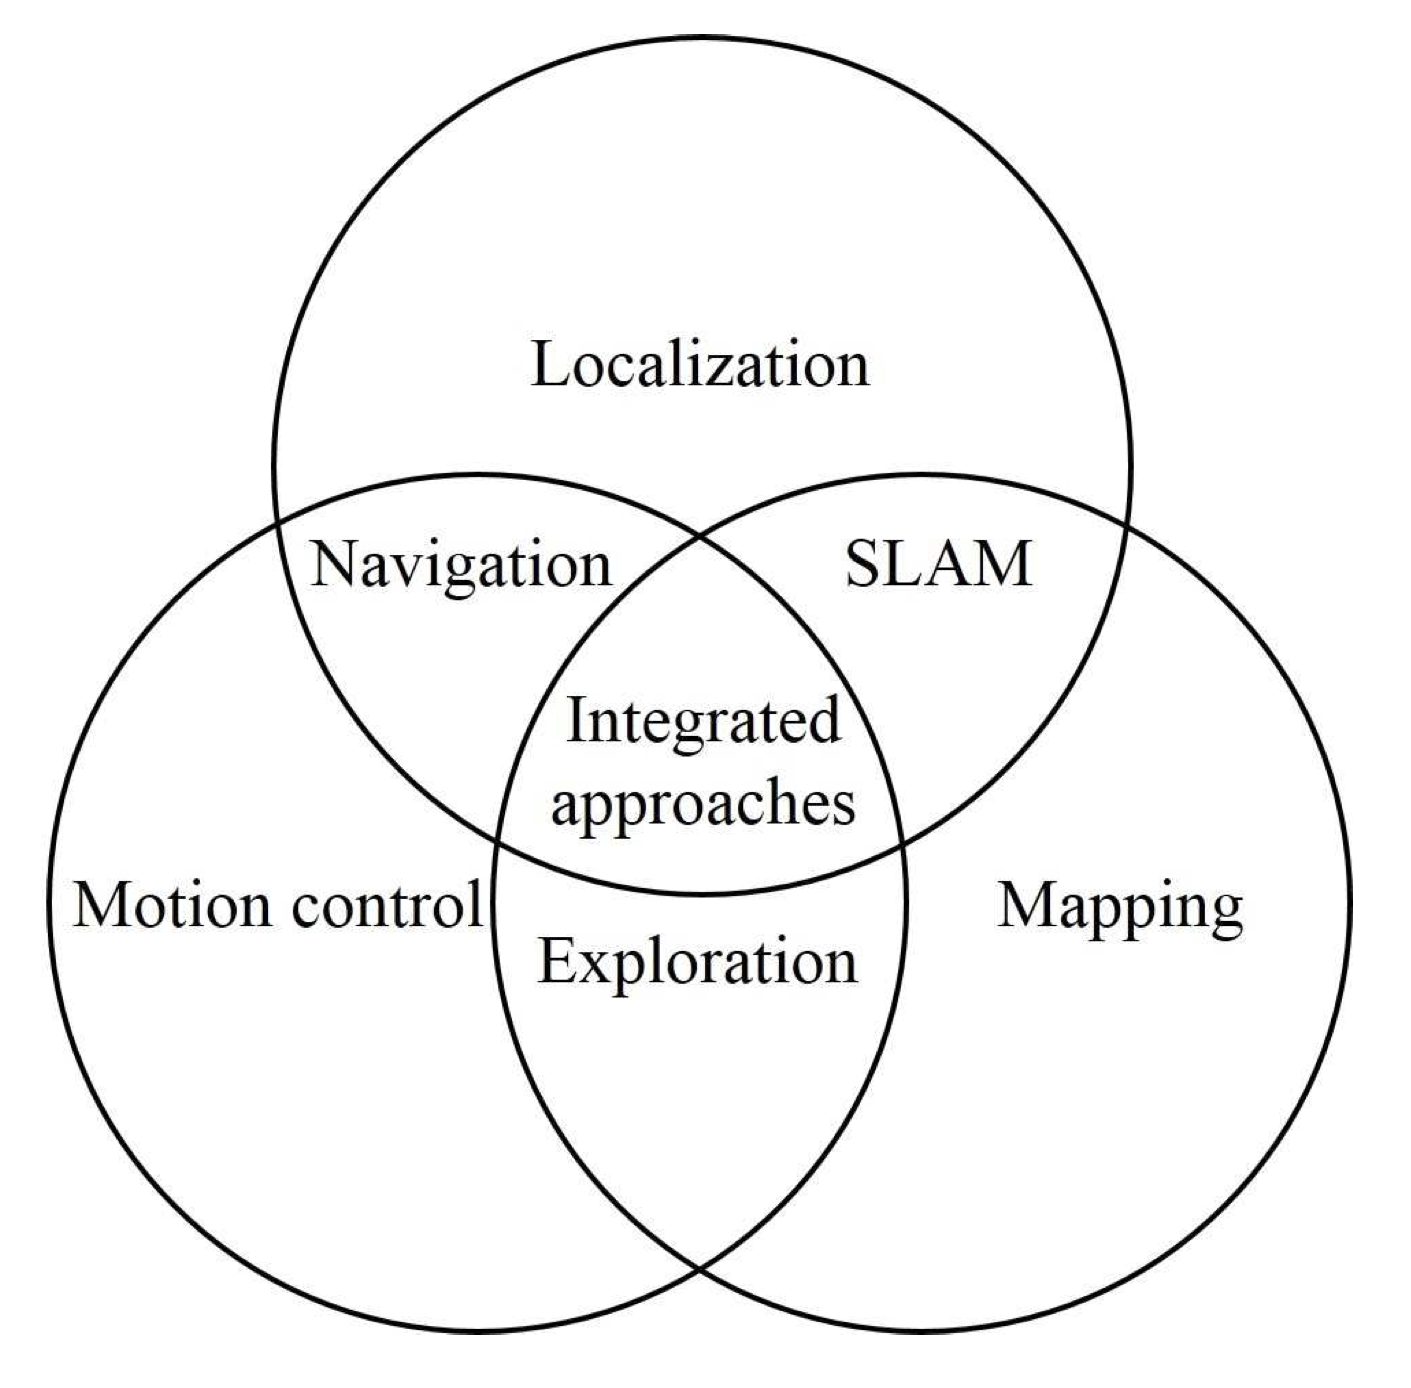
\includegraphics[width=0.5\linewidth]{fundamental-technology-3.png}
  \caption{Fundamental technologies for autonomous mobility\cite{赤井直紀2016自律ナビゲーションにおける}}
  \label{fig:fundamental-technology}
\end{figure}

ロボットが自律移動を行う際に必要となる最も基本的な技術要素は，自己位置推定(localization)，地図作成(mapping)，動作計画(motion control)の３つである．
自己位置推定は，事前に作成された環境地図をもとに，センサによる観測値と比較・照合をすることで，ロボット自身が与えられた環境地図上のどの地点に存在するかを特定する技術である．
地図作成は，ロボットが未知の環境を走行中にセンサから取得した観測値に基づいて環境地図を構築する技術である．
動作計画は，ロボットが環境地図上で自己地位推定を行いながら目的地へ向かうための経路計画を行う技術である．
本研究では，人が混在する動的な環境や駐車場などの環境変化が起きやすい実環境において，正確かつ安定した自律移動を実現することを主目的としているため自己位置推定の関連研究について述べる．

\section{自己位置推定について}
内界センサを用いた自己位置推定では，既知の初期位置からの移動量を逐次積算することにより，移動ロボットのおおよその位置を求めることができる．
内界センサには，車輪の回転量を計測するエンコーダや，角速度や加速度を計測するInertial Measurement Unit（IMU）などが用いられる．
これらのセンサから得られた移動量や角度変化を逐次積算することで自己位置推定を行う手法をデッドレコニングと呼ぶ．
しかし，エンコーダによるホイールオドメトリでは，路面の凹凸やひび割れ，あるいは路面上の破片などによる非系統的オドメトリ誤差や，左右の車輪直径の違い，トレッド幅の誤差などによる系統的オドメトリ誤差により，長距離走行において自己位置推定誤差が累積する\cite{borenstein1996measurement}．
また，IMUを用いた慣性航法では，ジャイロセンサや加速度センサのバイアス誤差，観測ノイズ，スケールファクタ誤差，温度変化や振動などの環境要因に起因する誤差の影響により，観測値の積分に伴って自己位置推定誤差が累積する\cite{borodacz2022review}．
そこで，ホイールオドメトリとジャイロセンサを融合したジャイロオドメトリが提案されている\cite{borenstein1996gyrodometry,前山祥一1997移動ロボットの屋外ナビゲーションのためのオドメトリとジャイロのセンサ融合によるデッドレコニング}．
ホイールオドメトリとジャイロセンサを融合することで，路面の凹凸によって生じる方位角誤差の低減や，ジャイロセンサのバイアス・ドリフトの推定および補正が可能となり，自己位置推定精度の向上が期待できる．
しかし，ジャイロオドメトリにおいても自己位置推定誤差の累積を防ぐことは困難である．
したがって，長時間かつ長距離の走行において高精度な自己位置推定を維持するためには，外界センサから得られる観測情報を用いて，内界センサによる自己位置推定の累積誤差を補正する必要がある．


外界センサを用いた自己位置推定手法の一つとして，GNSSを用いた測位が挙げられる．
GNSSは，人工衛星から送信される電波を利用して絶対位置を取得する測位システムであり，屋外環境において移動ロボットや自動運転車両の自己位置推定に広く利用されている．
しかし，GNSSは高層建築物などによる衛星電波の遮蔽や反射によって，マルチパスやNon-Line-of-Sight(NLOS)が生じ，測位精度が低下するという問題がある．
都市部におけるGNSS信号の遮蔽およびマルチパスの模式図を\cref{fig:multipath}に示す．
\begin{figure}[htbp]
  \centering
  \begin{subfigure}[b]{0.38\linewidth}
    \centering
    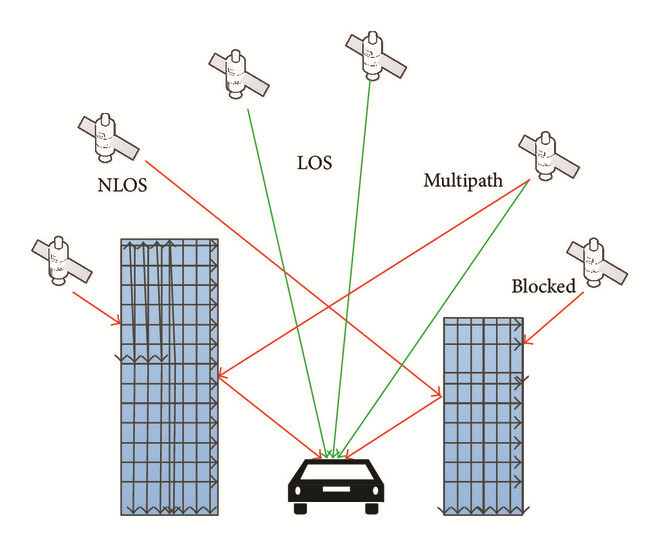
\includegraphics[width=\linewidth]{multipath.jpg}
    \caption{Front view}
    \label{fig:multipath-front}
  \end{subfigure}
  \hfill
  \begin{subfigure}[b]{0.38\linewidth}
    \centering
    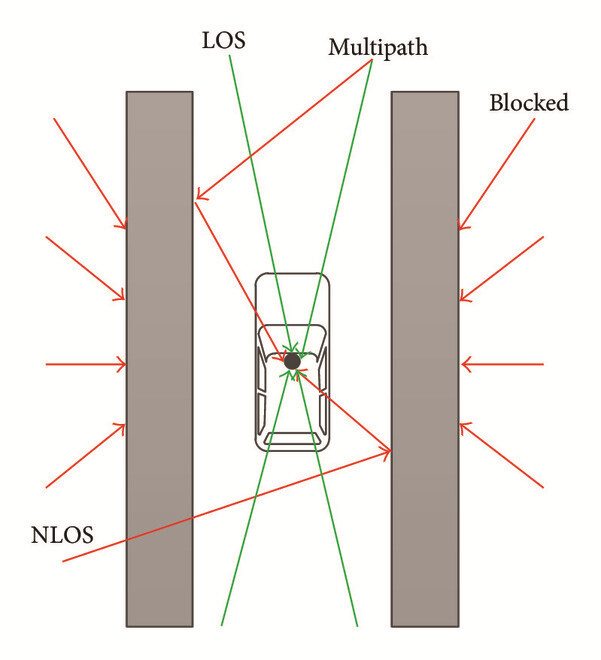
\includegraphics[width=\linewidth]{multipath2.jpg}
    \caption{Top view}
    \label{fig:multipath-top}
  \end{subfigure}

  \caption{Illustration of NLOS and multipath interference
  in urban canyons\cite{li2017tightly}}
  \label{fig:multipath}
\end{figure}
このような問題に対して，カルマンフィルタやパーティクルフィルタなどの確率的な推定手法を用いた自己位置推定が研究されている．
Liらは，GNSSと車載センサの観測情報を適応型ファジーアンセンテッドカルマンフィルタ(AF-UKF)によって統合する自己位置推定手法を提案した\cite{li2017tightly}．
この手法では，GNSSと慣性センサなどの情報を統合するとともに，衛星ごとの受信状態に応じて観測ノイズ共分散を適応的に調整することで，マルチパスやNLOSの影響を低減している．
また，Suzukiは，GNSSの擬似距離残差を利用してNLOS信号を検出し，Line-of-Sight(LOS)信号のみを用いて求めた位置推定結果と各パーティクルとのマハラノビス距離に基づいて尤度を評価する手法を提案した\cite{suzuki2019mobile}．
実際の都市環境における走行実験により，従来のGNSS単独測位と比較して自己位置推定精度が向上することを示した．
しかし，これらの手法によってマルチパスやNLOSの影響を低減できるものの，衛星電波の受信状態に依存するため，位置推定精度が低下する可能性は残る．
また，屋内環境では衛星電波の遮蔽や減衰によって十分な信号を受信できないため，GNSSによる自己位置推定は困難である．

\section{不可視地図を用いた自己位置推定について}

\section{センサーフュージョンについて}

\section{位置推定の失敗検知および復帰について}

\section{おわりに}
% \section{本研究の位置付け}
\label{sec:positioning}

本研究の位置付けを書きます．ささささささささささささささささささささささささささささささささささささささささささささささささささささささささささささささささささささささささささささささささささささささささささささささささささささささささささささささささささささささささささささささささささささささささささささささささささささささささささささささささささささささささささささささささささささささささささささささささささささささささささささささささささささささささささささささささささささささささささ．